%%%%% Change the four parameters in the line below:
% First is lecture #.
% Second is lecture title.
% Third is lecturer (either Anupam Gupta or Ryan O'Donnell).
% Fourth is your name.
\graphicspath{ {./2/} }
\lecture{2}{Graph Theory And Application}{Anand Misra}{Satya Prakash Sharma}

\section{Connection in Graphs}

\subsection{Walk}
A Walk in a graph is a sequence of edges such that each
edge (except the first one) starts with a vertex where
the previous edges ended. i.e The length of a walk is number of edges in it.

\paragraph{Path-}A path is a walk where all edges are distinct(no repeated edges).

\paragraph{Simple Path-}A simple path is a path where all vertices are distinct

\paragraph{Cycle-}A cycle is a path in which first and the last vertices are
same.

\paragraph{Trail-}A trail is a walk with no repeated vertex.


\subsection{Connected and Disconnected Graph}
A graph is \textbf{connected} if there is path between any two
pair of vertices in that graph. Otherwise it is
\textbf{disconnected}.


\paragraph{Connected component} of Graph G is maximal connected
subgraphs of G. (in other words, those connected
subgraphs which are not contained in larger connected
subgraphs of G.)


\paragraph{Connected component} of Graph G is maximal connected
subgraphs of G.


\subsection{Union of graphs}
The union of graphs G1,G2,..,G\textsubscript{k} written as \(\cup_{i=1}^k \)G\textsubscript(i) is the graph
with vertex set and edge set \(\cup_{i=1}^k \)V(G\textsubscript{i})

\paragraph{Proposition}
\begin{itemize}
    \item \textbf{Every graph with n vertices and k edges has
    at least n-k components}. - Since k edges can connects maximum of k+1 nodes and formed 1 component, 
    so here we have now n-(k+1) nodes remaining which forms n-(k+1) components, so in total we have 1+n-(k+1)
    i.e n-k. Therefore, Every graph with n vertices and k edges has
    at least n-k components
\end{itemize}

\subsection{Cut Vertex and Cut Edge}
\paragraph{Cut Vertex-}A cut-Vertex of a graph is an vertex whose deletion
increases the number of components.

\paragraph{Cut Edge-}A cut-edge of a graph is an edge whose deletion
increases the number of components.


\subsection{Theorem}
\begin{itemize}
\item \textbf{An edge is a cut-edge if and only if it belongs to no cycle.}
Take any edge e = {u, v}. Remove this edge from our graph: if the graph is still
connected, then there is some path from u to v not involving e; consequently, if we add e
to the end of this path, we get a cycle. Thus, if e is not a cut-edge, it’s involved in a cycle.


Conversely: suppose that e = {u, v} lies in a cycle. Let P be the path from u to v that
doesn’t use e (i.e. go the other way around the cycle.) Pick any x, y in G; because G is
connected, there’s a path from x to y in G. Take this path, and edit it as follows: whenever
the edge e shows up, replace this with the path P (or P traced backwards, as needed.) This
then creates a walk from x to y; by deleting cycles, this walk will always become a path,
and thus G is connected. So if e is involved in a cycle, it’s not a cut-edge.

\item \textbf{Every closed odd walk contain an odd cycle.}
    Let l be closed odd walk, For l=1, obviously true. (self loop).
    \textit{Suppose it is true for l<L, then we have to show that this is also true for L.}


    \textbf{Case1:} If there is no repetition of vertex in walk, then a closed walk = a closed cycle.


    \textbf{Case2:} If there is repetition in vertex in the walk, and let us suppose v is
    vertex which repeats. Break the walk into two v-v walks (say w1 and w2).
    Since |w1| + |w2| = odd, that means either w1 or w2 is odd walk. And surely
    they both are less than L. From the induction one of them (odd walk one)
    contain odd cycle.

\item \textbf{A closed even walk need not contain a cycle.}
    Example: If I go to jodhpur from my home and return back to my home from jodhpur with the same 
    route and it will count as a closed even walk, but it is not a cycle because \textit{ cycle is 
    a path in which first and the last vertices are same, and path has not repeated edges}

\end{itemize}






\section{Bipartite Graph}
A \textbf{bipartition} of a graph is a specification of two disjoint
independent sets in G whose union is V(G). The statement
“G is a bipartite graph with bipartition X and Y” specifies
one such partition.

\subsection{Proposition}
\begin{itemize}
    \item \textbf{A simple path is a bipartite graph.}- We can build a bipartite graph by have first node in 1 set and next to first in other set and do same for next to next as well.
    \item \textbf{A Cn is bipartite iff n is even.}- If n is even then then We can build the bipartite graph using first logic(A simple path). Similary, If Cn is bipartite graph then it must have n==even if n is odd then we can not put them in two set.
\end{itemize}


\subsection{Theorem}
\begin{itemize}
    \item \textbf{A graph is bipartite iff it has no odd cycle.}
    

    \textbf{Necessary condition:} Assume graph is bipartite and X and
    Y are two independent sets. To have a cycle, one has to
    traverse X to Y to X or Y to X to Y one or more time. 
    Therefore, a bipartite graph can't have odd cycle.

    \textbf{Sufficient condition:} If G has no odd cycle => it does not
    contain a cycle OR it contain even cycle.
    \begin{itemize}
        \item If does not contain a cycle : take one vertex in X and next verxtex in Y.
        \item If it contain even cycle : Partition the
        graph such that each even length cycle is one subgraph.
        We know Cn is bipartite for even length cycle.
    \end{itemize}
\end{itemize}



\section{Eulerian Circuit}

\paragraph{Eulerian Graph-}A graph is Eulerian if it has a closed trail containing all
the edges. We call a closed trail a circuit when we do not specify the
first vertex but keep the list in cyclic order.

\paragraph{Eulerian Circuit-}An Eulerian circuit in a graph is a circuit containing all the
edges.

\paragraph{Lemma-}If every vertex of a graph has degree at least 2, then G
has cycle.

\subsection{Theorem}
\begin{itemize}
    \item \textbf{A graph G is Eulerian iff it has at most one
    non-trivial component and all its vertices have even degree.}

    \textbf{Necessary condition:} Assume a graph G is Eulerian.
    \begin{itemize}
        \item It has closed trail containing all the edges.
        \item There will be an incoming and outgoing edge for all the vertices.
        \item All its vertices have even degree. (It has to have one non-trivial
        component, as more than one components closed trail might not
        be possible).
    \end{itemize} 

    \textbf{Sufficient condition:}  Assume a graph G has at most one
    non-trivial component and all its vertices have even degree.
    \begin{itemize}
        \item If number of edges m = 0 then G is Eulerian.
        \item \textit{Assume this is true for all graphs having less than M edges and
        obviously above properties. Then}
        \item Each vertex has at least two degree.
        \item G contains cycle (According to above Lemma). say C. Remove E(C) from G to construct G’.
        \item G’ has less than M edges and Each vertex of G’ has even degree.
        \item It can have more than one component. 
        \item By the induction hypo. Each component of G’ contain Eulerian Cycle.
        \item We combine these Eulerian cycles with C to construct an
        Eulerian circuit as follows: Traverse C until a component of G’s
        appear, then traverse Eulerian cycle of that component, come
        back to C and repeat this.

    \end{itemize}    
\end{itemize}
\begin{center}
    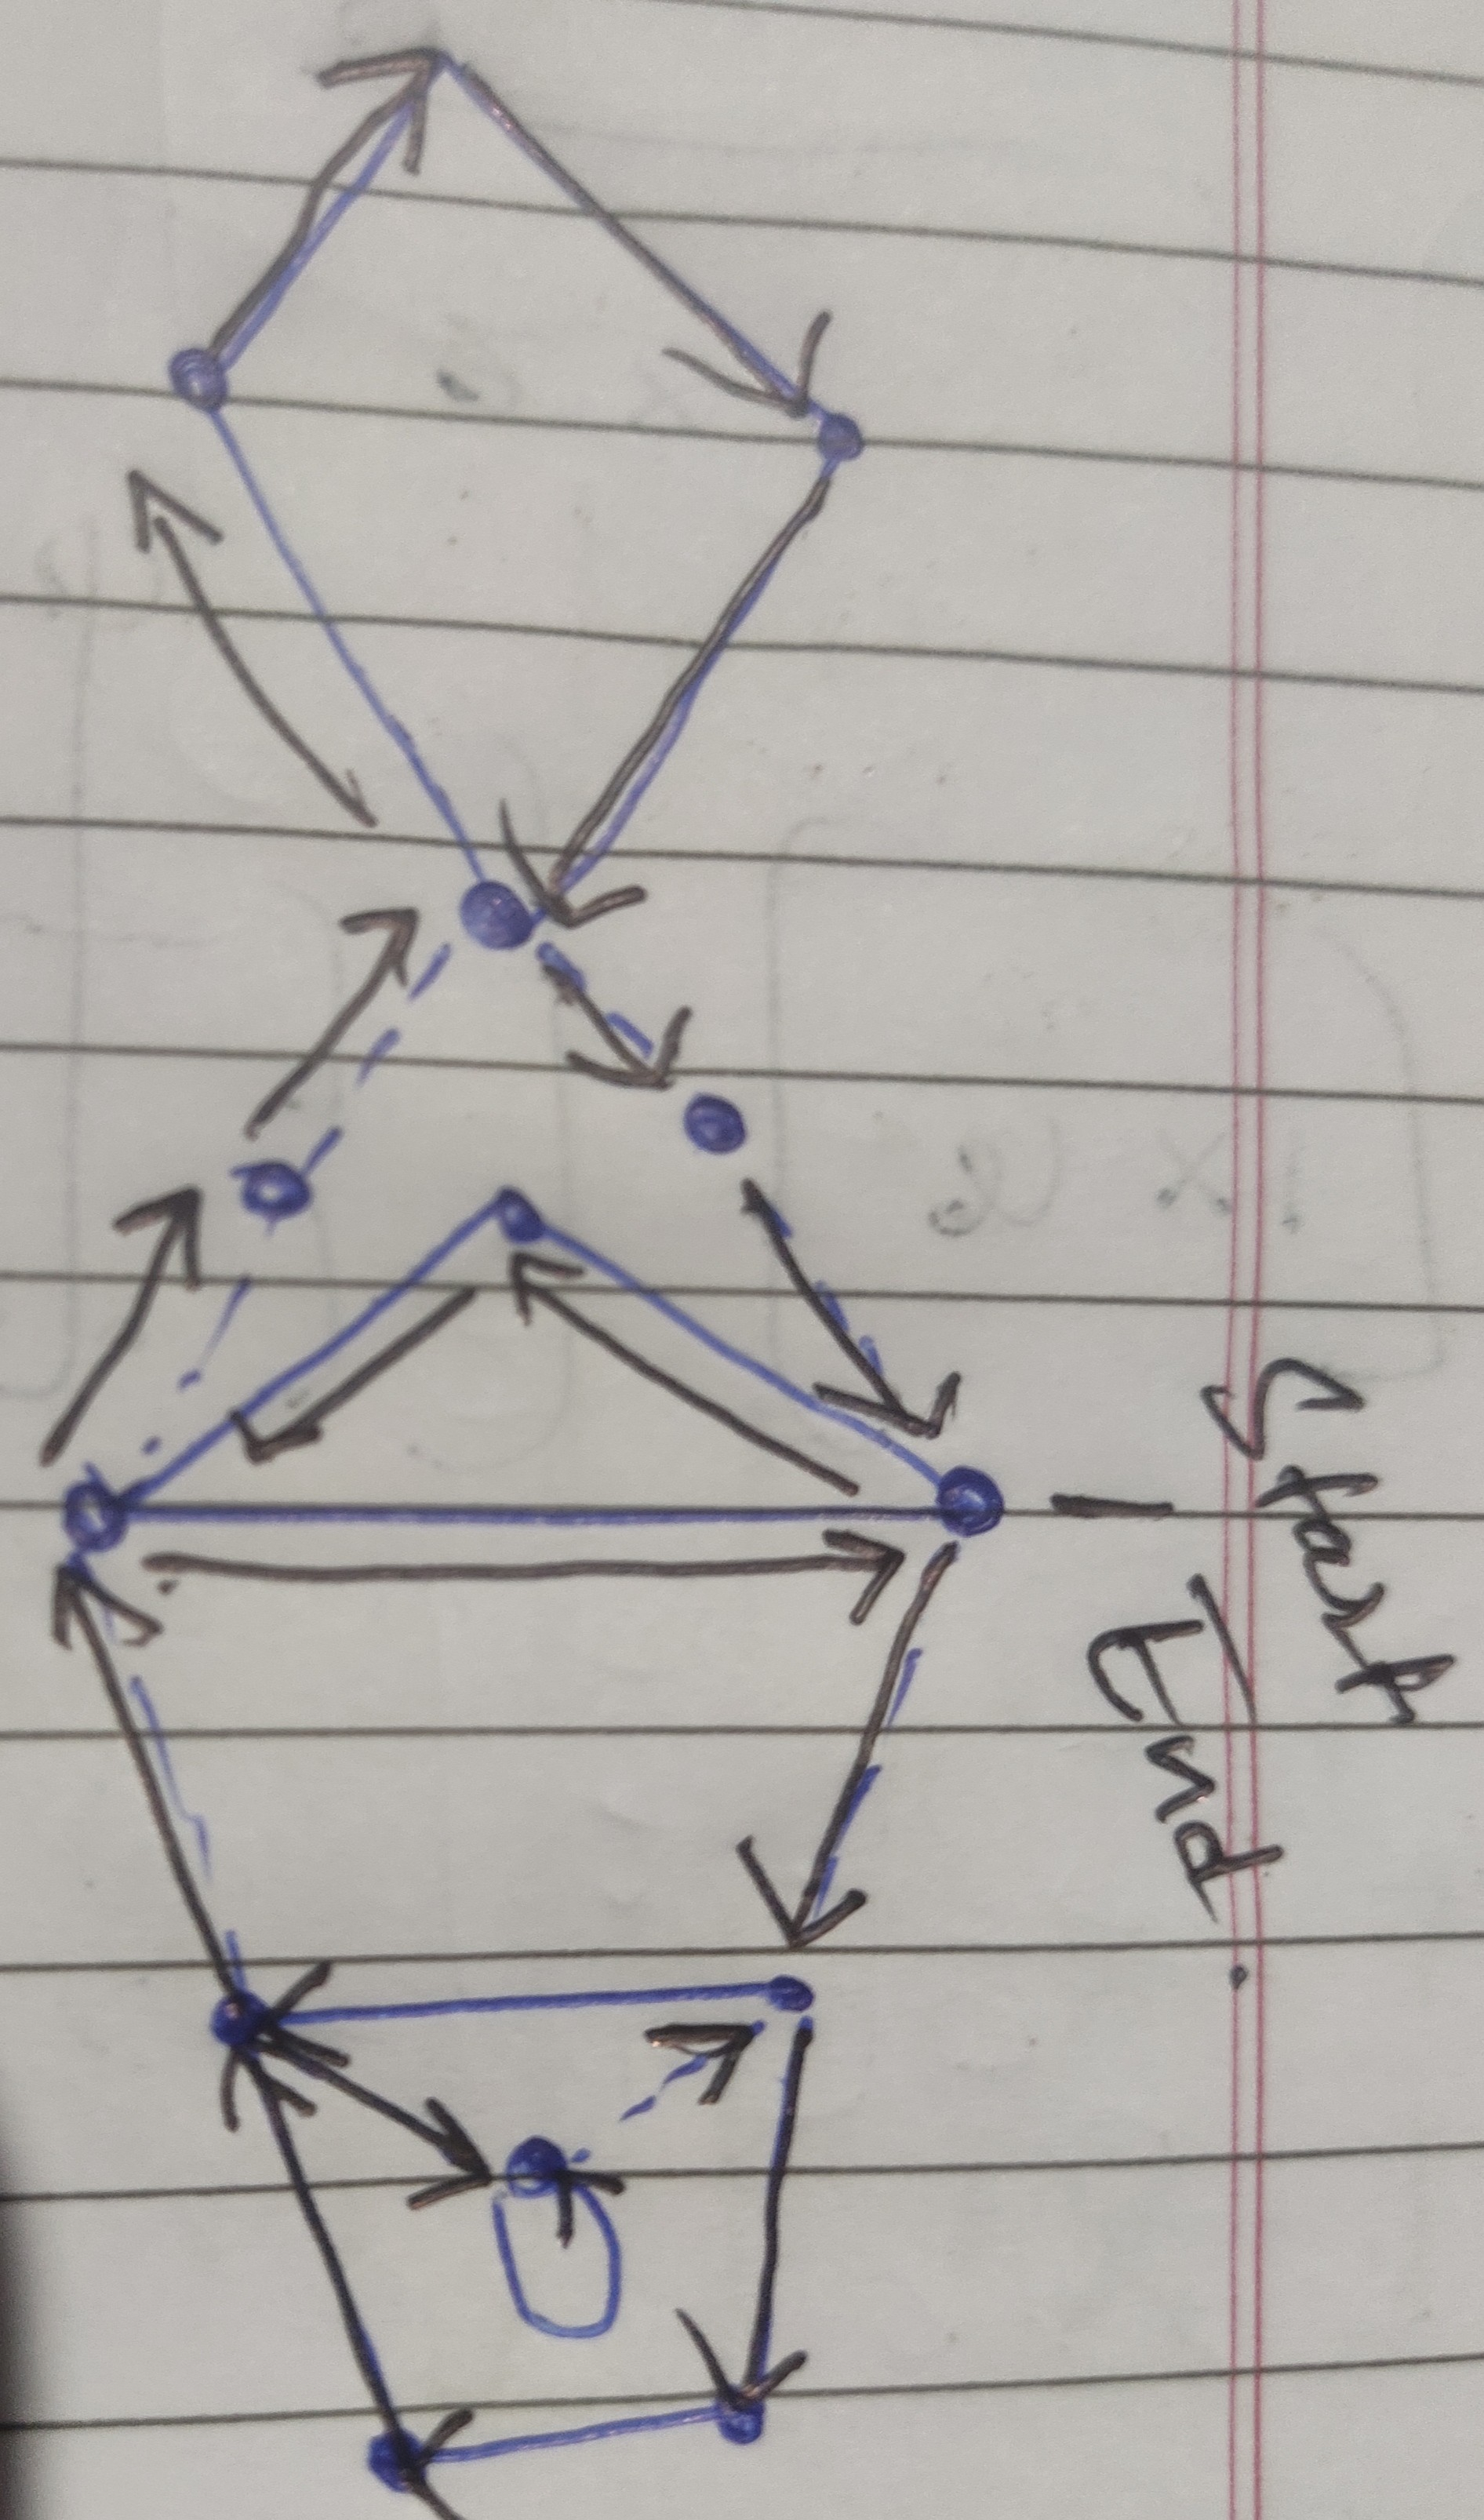
\includegraphics[scale=0.1, angle=-90]{eular_circuit}
\end{center}



\section{Vertex Degree and Counting}
\paragraph{Degree of a vertex-} Degree of a vertex v in a graph G written as d(v) is
number of edges incidents to v, except that each loop at v
counts twice. The maximum and minimum number of \( \delta(G) and \Delta(G)\)
degrees are denoted by respectively.

\paragraph{Order of Graph}The order of a graph G, n(G) is number of vertices in G.

\paragraph{Size of Graph}The size of a graph G, e(G) is number of edges in G.

\begin{itemize}
    \item \textit{The order and size of complete graph Kn: nC\textsubscript{2}}
    \item \textit{The order and size of complete bipartite graph Km,n: m*n}
\end{itemize}


\subsection{Handshaking Lemma} 
If G is a graph then \[ \sum_{v\epsilon V(G)} d(v)=2e(G) \]

\textit{Let G = (V, E) be a graph and let C be a connnected
component of G. Place one coin on each node in C for
each edge in E incident to it. }


Notice that the number of coins on any node v is equal to deg(v).


\textit{We claim that there are an even total coins distributed
across all the nodes of G.}


Notice that each edge contributes two coins to the total, one for each of its
endpoints. This means that there are 2m total coins
distributed across the nodes of V, where m is the number
of edges adjacent to nodes in C, and 2m is even.
Since there are an even number of coins distributed
across the nodes, our earlier theorem tells us that the
number of nodes in G with an odd number of coins on
them must be even. The number of coins on each node is
the degree of that node, and \textit{therefore there must be an
even number of nodes of odd degree.}


